\section{Introduction}
% Broad scope approach-motivation statement \\
% Funnel into short abstract-like summary of the project \\
% background in three sections: biohybrid BCI, direcitonal networks, MOT \\
% research problem, research aims + presented solution,  significance + which value \\


% Why do we need directional neural networks?
%     general entry funnel
%     biohybrid interfaces
%     disease models (sprinkle of bottom up neuroscience)

% which efforts have been made to make networks directional?
%     orient to csabas paper

% Which solution does this work provide?
%     primitives screen
%     20 test structures screen

% In this work, \dots [abstract like but shorter]

\subsection{Biohybrid neural interfaces}
Neuroelectric interfacing based on metal electrodes has made remarkable progress
over the last decades (\cite{utaharray}, \cite{neuropixel}). These technologies
excel at locally confined high resolution neural recording for a time period on
the order of weeks. However, given the immense challenges related to high
quality neural interfacing \parencite{mooreslaw}, naturally, existing recording
and particularly stimulation technology exhibit shortcomings.
% # clearly say that stimulation works worse than recording
The clinically most adapted CNS stimulation method, deep brain stimulation
(DBS), does not specifically depolarize single neurons but instead exerts
various modulatory effects on entire brain areas \parencite{dbs}. Low
spatiotemporal resolution may be tolerable for common DBS applications, however,
addressing the clinically highly relevant cases of vision-, touch-, or hearing
loss is currently limited by insufficient resolution
\parencite{retinastimulation}. Another issue affecting both stimulation and
conventional neural recording systems is the induced foreign body response. Due
to natural brain movement, rigid metal electrodes cause inflammation, neuronal
cell death and glia formation while simultaneously, conventional electrode
insulation undergoes biodegradation resulting in decreased impedance
(\cite{eletrodeproblems1}, \cite{eletrodeproblems2}, \cite{eletrodeproblems3},
\cite{eletrodeproblems4}). In research applications, central nervous system
(CNS) stimulation is most commonly performed through optogenetic tools
(\cite{optog1}, \cite{optog2}). While the cell-type specificity of optogenetics
can be of great value, the limitations in spatial resolution inherent to
\textit{in vivo} light-based technology seem to be a major hurdle for increasing
spatial resolution. On top of this, the risk of genetic off-target effects and
adeno associated virus (AAV) immune responses restrict medical use cases in the
near term \parencite{optogImmunresponse}. \\

Biohybrid implants take a fundamentally different approach to neural
interfacing, drawing inspiration from tissue engineering and \textit{in vitro}
neuroscience. First described by \cite{biohybridfirst}, this promising
technology aims to solve the latent issue of biocompatibility by moving towards
the integration of biological components \parencite{biohybridreview}. At the
same time, biohybrid technology may benefit from the highly impressive
\textit{spec sheet} of a neuron, including energy efficiency, self-containment,
and signal transmission properties. Whilst engineering with neural tissue
presents almost daunting challenges, the biocompatibility prospects of biohybrid
interfaces are currently inaccessible by competing technologies. CNS
applications of the biohybrid approach include the coating of metal electrodes
with host cells (\cite{seededelectrodes1}, \cite{seededelectrodes2}), and the
use of ectopic axons as electrodes (\cite{filmbasedinterface},
\cite{cullenrecent}). The currently most advanced biohybrid implant is based on
a hydrogel microcolumn containing ectopic cortical axons that are optogentically
driven through a light emitting diode (LED) optical fiber outside the brain
\parencite{cullenrecent}. While synapse formation was shown anatomically
\textit{in vitro}, the \textit{in vivo} proof-of-concept implantation did not go
as far as showing functional target tissue innervation. \\

\begin{figure}[h!]
    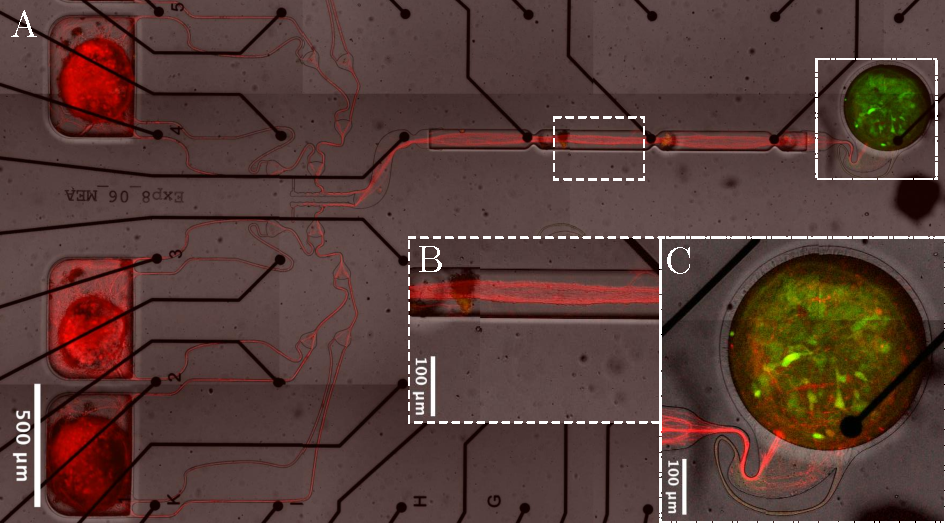
\includegraphics{I_thal_innervation.pdf}
    \caption[DIV 17 biohybrid implant assembled on glass MEA]{DIV 17 biohybrid
        implant assembled on glass MEA. \textbf{A} Confocal image of a biohybrid
        implant 17 days after seeding (DIV 17). Rat E18 RGC spheroids were
        labelled with mRuby (red), the E18 rat brain target was labelled with
        GFP (see Methods for details). Black lines in the transmission channel
        mark the PDMS micro structure. Only 3 of 4 RGC seeding wells are
        shown. \textbf{B} Magnification of the output channel with a grown nerve
        bundle. \textbf{C} Magnification of stomach target structure showing RGC
        innervation of E18 rat spheroid.}  
    \label{I_thal_innervation}
\end{figure}

Current biohybrid implants trade off biocompatibility for interface bandwidth
and control. For example, the biohybrid implant presented in \cite{cullenrecent}
relied on optically exciting the entire ectopically grown neural population,
resulting in limited control of delivered stimulation. While this spatial
resolution may be sufficient for specific use cases, this implant design offers
insufficient control for delivering high dimensional data, such as sensory
input. For addressing the pressing issue of functionally restoring sensory
modalities \parencite{blindnesssux}, a biohybrid implant needs to allow for
stimulating independent channels. To solve this crucial design requirement, the
implant presented here is based on a PDMS micro fluidic system enabling the
independent stimulation of axons grown in micro channels. Briefly, PDMS
membranes are placed on coated glass dishes or multi electrode arrays (MEA) and
seeded with E18 rat RGC spheroids (Figure \ref{I_thal_innervation} A). Axons
extend through the 6 $\upmu$m high channel system until they reach the 3 mm long
output channel which will eventually be implanted (Figure
\ref{I_thal_innervation} B). The final device will utilise stretchable
AuTiO\textsubscript{2} nanowire electrical contact pads for stimulating RGC
axons \parencite{nanowires}. Long term host cell survival will be ensured by
having the implant face the brain surface such that RGC spheroids are integrated
with the CNS microenvironment. The device will be implanted targeting the dorsal
lateral geniculate nucleus (dLGN), although currently, the implant is optimized
\textit{in vitro} targeting E18 rat brain spheroids (Figure
\ref{I_thal_innervation} C). 



\subsection{Engineered directional neural networks}
It is well established that the connectivity within biological neural networks
is a major determinant of the emerging electrophysiological dynamics. For
example, the canonical microcircuit of the cat visual cortex exhibits a high
degree of sparsity with predominantly local inhibitory-, and excitatory
connections to achieve its output \parencite{ctxcircuit}. Despite the general
agreement on the significance of neural circuits, the vast majority of
\textit{in vitro} models remain limited to random connectivity schemes.
Neglecting this property of \textit{in vivo} neural networks may be well
justified in studies that focus on basic biological properties, for example in
response to drug admission. However, any model system investigating higher level
functional properties emerging at the circuits-level (e.g. learning mechanisms)
requires confined connectivity. \\

More elaborately controlled connectivity schemes are indispensable for
technology relying on living neural circuits. Biohybrid interfaces as described
above rely fundamentally on directional connectivity (Figure
\ref{I_thal_innervation} A). Innervation of neighboring RGC source wells may
result in activity dynamics independent of the imposed electrical stimulation
pattern, rendering single stimulation channels or the entire device unusable.
For this reason it is crucial for viable biohybrid implants to achieve high
degrees of growth directionality. \\
Likewise, more sophisticated models focusing on functional aspects of the
peripheral nervous system (PNS) may benefit from directional \textit{in vitro}
models. PNS circuits generally show a pattern where sensory-, or motor axons
converge to form a nerve that eventually diverges again in the target location.
Building an \textit{in vitro} platform resembling this architecture would be
extremely useful for studying neuropathy, traumatic nerve injury, and tissue
reinnervation. The canonical design of the biohybrid implant where multiple RGC
source nodes converge into a common output channel replicates this motif. \\

% While pathological questions regarding the nerve itself may be investigated with
% artificial nerve models of limited directional connectivity
% \parencite{3dnervemodel}, functionally more complex pathologies, for example
% those related to development require directionally constraint in vitro models.
% \\

The challenge of achieving directional \textit{in vitro} networks is often
reduced to imposing axonal or dendritic growth constraints once the neurons are
seeded. Although it is conceivable that initially randomly connected neural
networks develop directional connections solely by an electrically imposed
activity pattern \parencite{stdp}, this approach has so far been to no avail.
Therefore, various \textit{in vivo} inspired approaches have been taken to
instead induce control on axonal outgrowth. Axon guidance mechanisms \textit{in
vivo} rely broadly speaking, on two categories of cues: structural and chemical
ones (\cite{mechanicalcues}, \cite{chemicalcues}). Chemcial cues have been
employed for guidance by integrating substrate surface modifications favoring
certain growth paths. Although many attempts are limited to micro patterning
with PDL falling short of the highly complex chemical micro environment observed
\textit{in vivo}, still, a notable degree of axonal growth control is achieved
\parencite{singlecellmCP}. While chemical guidance remains a promising direction
for engineering defined neural networks in the future, structural guidance has
shown more promising results at larger network scales \parencite{forro}. 

The idea of utilizing structural growth guidance \textit{in vitro} is largely
based on advances in microfluidics for neuroscience (\cite{microfludics1},
\cite{microfludics2}).  These platforms are commonly fabricated from PDMS, a
polymer that can be molded at high resolution using soft lithography, while also
exhibiting acceptable biocompatibility properties \parencite{pdms}. 3D
structural guidance principles are based on the inertia of growing axons, e.g.
the inability to grow in sharp turns, and the tendency of axons to attach to
edges \parencite{axongrowth3d}. These two findings are the basis of numerous
PDMS design motifs proposed in the literature to achieve directional growth
through PDMS micro structures: barbed-, and narrowing channels, (\cite{lefeber},
\cite{peyrin},) redirecting hooks and consecutive arches (\cite{pirlo},
\cite{na}, \cite{renault}, \cite{2019afterForro}), and diode-like triangles
(\cite{gladkov}, \cite{isomura}). So far, the most competitive multi node
directional networks are based on a relatively simple motif, where axons detach
from sharp radii and thereby avoid growth in the undesired direction
\parencite{forro}. \\

While \cite{forro} presented respectable results for four-node-networks, the
nerve model system and surely the biohybrid implant require an order of
magnitude more nodes, while also deviating from the rather simple one-to-one
connectivity scheme. In this work we present a high resolution screen on the
growth directionality in 21 many-to-one PDMS designs. To the best of our
knowledge, no networks have been shown to merge as many as 32 source nodes into
a common target node. Since directional axon growth through PDMS micro
structures is a probabilistic process, the addition of nodes increases the
relative chance of non-directionally connected cultures. 

\subsection{Multiple object tracking}
In this work, we employ a custom build, machine learning-based growth cone
tracking model to screen PDMS micro structures for directional growth. Previous
work has relied on screening network directionality electrophysiologically
(\cite{forro}, \cite{isomura}, \cite{lefeber}), through calcium indicators
\parencite{na}, manual-, or segmentation based axon counting (\cite{pirlo},
\cite{forro}) and by calculating fluoresce intensity ratios (\cite{renault},
\cite{na}). Due to the general geometrical complexity and the multitude of
junctions within our micro structure designs, previously employed
anatomically-based screening methods did not meet our requirements.
Alternatively, functional screening methods offer high resolution, but are often
limited to low experimental throughput. For those reasons, we resorted to
tracking growth cones during the initial outgrowth phase, yielding a high
resolution, anatomically-based estimation of directionality. \\

The problem of multiple object tracking (MOT) consists of identifying objects
and linking their identities over multiple video frames, either offline with the
entire sequence available, or online where future frames are not observed.
Extensions of this include the classification and segmentation of identified
objects. With notable exception \parencite{graphmot}, this problem has been
divided into object detection and identity association. Since the seminal paper
by \cite{alexnet} introducing the concept on learned convolution kernels, object
detection has been increasingly dominated by machine learning based detectors.
While the architecture of an image classifier is straight forward, mapping from
the image pixel map to the number of classes, object detection deals with an
unknown number of instances within an image, making it unclear what the network
output shape should be. The first solution to this problem was the regions
convolution neural network (R-CNN) architecture by \cite{rcnn},
implementing the recurrent classification of small image regions (for improved
versions see \cite{fastrcnn}, \cite{fasterrcnn}). The inherently low inference
speed in these architectures was addressed by the \textit{you only look once}
(YOLO) architecture by dropping the recursive aspect completely (\cite{yolo},
\cite{yolo3}, \cite{yolo5}). The ensuing step of data association has been
dominated by non machine learning based methods (\cite{sort}, \cite{hungarian},
\cite{MCF}), although deep learning alternatives have recently been proposed as
well (\cite{deepsort}, \cite{assreview}). \\

In the biological microscopy literature, the above is often found under the term
\textit{particle tracking}, indicating the focus on small objects such as cells,
organelles, or proteins (\cite{celltracking}, \cite{organelltracking},
\cite{proteintracking}). Although the general problem matches the outline above,
tracking of biological objects such as growth cones generates a specific set
of additional challenges. Concretely, the setup used for screening PDMS micro
structures imposed the following: (i) Objects of interest, i.e. growth cones are
often extremely small, thus conventual CNN architectures based on hierarchical
feature extraction of larger objects are not suitable. (ii) Microscopy images
are taken at very high resolution, raising computational demands. (iii)
Inter frame intervals are long, here around 30 minutes, (iv) Growth cone
appearance is highly variant; growth cones can overlap and collapse abruptly.
(v) No labelled dataset exists, and widely available pretrained models
generalize poorly. Our tracking implementation is build on established methods
with modifications addressing the points i-v. For more details see methods
\ref{modeldescription}. \\



% Deep learning has been explored for video tracking of objects such as vehicles,
% people and animals (Bertinetto et al., 2016; Leal-Taixé et al., 2016; Ning et
% al., 2017). However, there are essential differences between particle tracking
% in time-lapse microscopy and object tracking in other video applications. First,
% particles are typically subresolution objects, which have little or no
% distinctive appearance features in the images, unlike objects such as cars and
% humans in videos, from which rich feature sets can be extracted that can be
% beneficial for tracking. Second, particles may appear or disappear anywhere in
% the field of view, whereas objects in video applications are more likely to
% enter or leave at the frame borders. Third, in many biological experiments, the
% number of particles to be tracked runs in the hundreds to thousands, which is
% orders of magnitude larger than in most other applications, where only a single
% or at most a handful of objects need to be tracked. And fourth, the temporal
% resolution of the image sequences is often relatively low in particle tracking
% as compared to other object tracking applications, to avoid photodamage and
% photobleaching. Thus, deep-learning methods for common single and multiple
% object tracking cannot be simply adopted for particle tracking.



% \subsection{(ABSTRACT FROM SHORT PROJECT)}
% Capable brain-machine interfaces are the foundation for progress in
% neuroscience research, medical treatment of the brain and thought provoking
% black mirror episodes. In Moore's law fashion, the density at which we can
% record single neuron activity \textit{in vivo} has doubled every seven years
% over the last 60 years (albeit partially ignoring spatiotemporal
% resolution). On the contrary, current electrode technology is incapable of
% stimulating multiple neurons at single cell resolution \textit{in vivo}. We
% will overcome this problem by employing a tissue-engineering approach:
% Instead of relying on metal electrodes limited to expansive stimulation, our
% biohybrid multielectrode array (bioMEA) uses \textit{in vitro} grown ectopic
% neurons whose axons innervate the region to stimulate. In simple terms, the
% implant consists of a PDMS (silicone) guidance microstructure that directs
% the ectopic axons into the implanted tube. Below the guidance channels is a
% stretchable electrode array that enables us to stimulate our neurons
% electrically and send action potentials to the implanted brain region. \\
% The initial motivation of the sub-project presented here emerged from
% criticism pointing out the overwhelm- ing complexity in engineering this
% biohybrid interface. Given the difficulties involved when building with
% biological parts, we asked how should one approach this complex engineering
% task such that chances of success are maximal. The answer provided by this
% work is a framework that decomposes the engineering process into sub
% components that are iteratively optimized using a high-throughput debugging
% platform. Due to the multitude of parameters to consider in our device, the
% efficiency at which we are able update the prototype is likely going to
% determine the success of the project. A significant amount of time was
% therefore invested in modelling new axon guidance structures. Crucially, the
% new layout of PDMS structures permits specialized experiments and testing
% with higher throughput. Moreover, the modelled PDMS mask includes 20 new
% implant designs that address the issue of non-directional growth through the
% guidance structure resulting in decreased bandwidth and cross-talk between
% electric channels. Incorporating channel connectivity, attractor cue
% gradients and specific guidance motifs into the design model, the new
% structures should exhibit highly improved directional axonal growth towards
% the implanted tube. All in all, this work shows the feasibility, and lays a
% foundation for building a stimulating biohybrid multielectrode array, ensued
% by taking first practical steps by designing a new PDMS wafer for
% fabrication.

% \subsection{High level overview (from short project)}
% This work is a contribution to the more comprehensive endeavor of building
% a brain machine interface using ectopic axons as electrodes. As this work
% addresses fine-grain engineering problems, one first needs to get a general
% overview of the device, its components, and the assembly process to
% appreciate the results presented here. Before going into the underlying
% details of the device though, we may want to ask why this is a relevant
% project to work on in the first place. At the lowest level, the device is
% motivated by the fundamental wall researchers and biomedical engineers face,
% regarding high-density stimulation of the brain with spatial resolution
% beyond large neural populations. \\
% While recording technologies have made considerable progress over the last
% years, stimulation methods have not kept up. In the medical domain, deep
% brain stimulation of basal ganglia has received a lot of attention over the
% last decade, especially due to the remarkable improvements for patients
% suffering from Parkinson disease (PD). Still, these systems suffer from a
% range of shortcomings: first and foremost, the spatial resolution of
% stimulation is limited to neural populations or entire nuclei, second,
% immunoreaction to the implanted electrodes causes complications in the long
% term, and lastly, these systems are limited in their adjustability post
% surgery, as voltage and pulse width are the only tunable parameters. In
% research applications, brain stimulation is dominated by optogenetic
% methods. Similar to electrical deep brain stimulation, this technology comes
% with spatial limitations imposed by the nature of light. On top of that,
% optogenetic stimulation requires genetic engineering in the target region,
% currently still a notable hurdle for any medical application. \\
% Our biohybrid multielectrode array (bioMEA) aims to achieve stimulation at
% single-neuron resolution while simultaneously resolving the latent issue of
% biocompatibility encountered with implanted metal electrodes. Such
% single-cell resolution interfaces are strictly required for delivering high
% dimensional information, for example from the sensory domain. This is the
% initial area of application we intend to target with this device,
% specifically, restoring the visual input to the dorsal lateral geniculate
% nucleus (dLGN) as depicted in Figure \ref{fig:overview} below. \\

% We prepare the implant \textit{in vitro}, with axons already
% inside the structure. The device is then implanted under the skull such
% that ectopic neurons face down to receive nutrients from the brain
% surface; the guiding axon channel terminates in dLGN. We hope that the
% combined effect of absent input from the optic nerve (dissected) and
% applying stimulation through the interface induces the formation of
% functional synapses. The animals age and the time interval from
% optic nerve dissection to implantation is likely to be critical for this
% to occur. In a final application, the interface is connected to a
% neuromorphic chip that functions as an artificial retina processing raw
% camera signals

% \noindent
% % To achieve this, we take a tissue engineering approach, trying to built
% % the device from mostly biological parts.
% How does the current prototype device work? We start by preparing the PDMS
% structures which house and guide the ectopic neurons. These 250 um x $\sim$2
% mm x $\sim$5 mm (z, x, y) structures implement the source wells for ectopic
% neurons from which 6 um high tracts extend out of. In the final device,
% these 6 um axonal tracts run over stretchable AuTiO\textsubscript{2}
% nanowire electrical contact pads that enable stimulation of neural
% electrical activity by depolarizing the axon above it. However since
% manufacturing these PDMS-based stretchable electrode arrays is challenging,
% we currently place our structures on glass multielectrode arrays
% (Multichannel Systems MCS GmbH) to measure and induce electrical activity.
% The 6 um axon channels connecting to the source wells converge into the 3 mm
% long output channel which will eventually be implanted. For optimal
% biocompatibility and fast growth, a nanofiber tube will be used for this in
% the future, but in the current design iteration we simply use a wider and
% higher PDMS channel. To attract axons towards this output channel, we place
% a piece of thalamic tissue on the 3 mm output channel (has small openings)
% so that emitted cues can diffuse into the PDMS structure. \\
% This PDMS 'lobe' is placed in a glass well (or the glassMEA when electrical
% interfacing is required) that has been coated with  laminin and
% poly-D-lysine to facilitate growth. In past designs, we seeded dissociated
% primary retinal ganglion cells (RGCs) obtained from E18 rat retinas, but for
% neural viability and simplicity reasons, we recently moved to larger source
% wells that house retinal tissue pieces of size 300 um x 300 um. Axons
% elongate at a speed of about 400 µm/day and usually reach the end of the 3
% mm long output channel within two weeks.


% \subsection{Low level overview (from short project)}
% As might be apparent from the outline above, building this bioMEA for neural
% interfacing is a challenging engineering problem with a multitude of
% potential obstacles in the way; it is not clear that our orthogonal approach
% to building a CNS stimulation device is tractable. Given the general
% unpredictability when doing engineering with biological parts, one may
% critically ask why this has a chance to succeed. In a way, the first results
% section of this report can be interpreted as answering a related, more
% productive question: how should this problem be approached if we aim for
% maximizing the probability of success? Coming from the very realization that
% we picked a difficult engineering problem, one motivation of this work was
% to come up with a systematic engineering process that at the end yields a
% working prototype. The prototype device should exhibit minimal cross talk
% between channels, RGC survival on a timescale of months, and most
% importantly, the ability to form functional synapses on thalamic tissue
% \textit{in vitro}. In \textbf{section \ref{framework}}, we formulate a
% simple engineering framework from which a potential experimental roadmap
% derives. This formulation of the engineering process enables one to split
% the problem in smaller, approachable tasks, allowing for iterative,
% parallelized optimization of isolated components. \\
% To effectively execute on the experimental plan that derives from this
% framework, new PDMS designs are indispensable. A central argument made by
% this report is that we need to move towards high-throughput, efficient
% experimental cycles to optimize the device on a reasonable timescale.
% Achieving this is strongly contingent on smart PDMS structure layouts that
% permit fast testing. Motivated by this assigned significance, one entire
% month of this three month project was dedicated to planning and modelling a
% new PDMS wafer, which is explained in \textbf{section \ref{general_design}}
% (remaining two months were spend learning practical protocols). We model the
% desired 2D channel structure in CAD using Fusion360, AutoCAD and KLayout.
% This design is rendered as a .gds2 file to create the fabrication mask. We
% send this mask design to Wunderlichips GmbH, a private company that
% fabricates the silicon wafer using SU-8 mold photolithography. The wafer has
% a diameter of $\sim$10 cm allowing us to arrange the single implant
% structures in a grid like pattern (see Suppl. Figure \ref{fig:wafer} for the
% complete new wafer design).\\
% Besides general optimization of the experimental throughput through the PDMS
% wafer design, this work describes 20 new PDMS structures and the conceptual
% model behind the design process \textbf{(section \ref{specifc_design})}.
% These specific implant designs aim to solve an immediate problem we
% currently experience with our PDMS structures: directional growth. Ideally,
% we want all axons originating from the source wells to grow into the tube
% that will eventually be implanted. However right now, a great number of them
% grow towards neighboring seeding wells. Incorporating optimal tract
% connectivity, cue gradients and PDMS motif designs in the design process,
% the new microstructure designs assure unidirectional axonal growth towards
% the implanted tube (in the final device made from nanofibers, right now
% PDMS). \\
% Note that due to length limitations, integration with existing literature
% and discussion are kept to a minimum. 



% \pagebreak